\documentclass[11pt,parskip=half,headings=small,german]{abnh}
\usepackage{pdflscape}

\geometry{a4paper, portrait, left=2.5cm, right=2cm, top=1.5cm, bottom=2.5cm}

\begin{document}

%\includegraphics[width=\linewidth]{logo.png}

\vspace*{0.5cm}

\begin{mdframed}[rightmargin=3cm]
\Large \textbf{\textsf{Abitur 2025 -- Nachprüfung im Fach Mathematik (LK)}}	
\end{mdframed}


\textsf{\textbf{Datum der Prüfung: } \hfill \textbf{Raum: }}

\vspace{1cm}

\begin{tblr}{
  colspec={|X[l]|X[l]|X[l]|X[l]|X[l]|},
  hlines,
  vlines,
  width=\textwidth,
  row{1-5} = {abovesep=4pt, belowsep=4pt}
}
\textbf{Prüflinge:} Name, Vorname &  & &  &  \\
\textbf{Uhrzeit:} &   & &   &   \\
\textbf{Prüfer: } &   & & &  \\
\textbf{Protokoll:}   & & &  \\
\textbf{Vorsitz:} &   & & &  \\
\end{tblr}

\vspace{1cm}

\textbf{Thema: }Analysis und Stochastik

Hilfsmittel:

\begin{itemize}
	\item ein Wörterbuch der deutschen Rechtschreibung
	\item eine Liste der fachspezifischen Operatoren
	\item Wissenschaftlicher Taschenrechner
\end{itemize}

Der Schwerpunkt der Prüfungsaufgaben liegt im Halbjahr Q1 (Thema: Analysis) und im Halbjahr Q3 (Thema: Stochastik).

\newpage

{\large \textbf{\textsf{Analysis}}}

\begin{abienum}
	\item Dietzenbach ist mit ca. 36000 Einwohnern auf Platz 23 der größten Städte Hessens. Während eines Volksfestes wurde ein seltenes Zombievirus in die Stadt eingeschleppt. Aktuell sind bereits 1000 Einwohner erkrankt. Man geht davon aus, dass sich wöchentlich 10\% der bisher noch nicht infizierten Einwohner anstecken.

	Drei Mathematiklehrer der Heinrich-Mann-Schule schlagen die folgenden drei Funktionen zur Modellierung der Gesamtzahl der erkrankten Einwohner (t in Wochen) vor:

\vspace{-0.5cm}

	\begin{align*}
		f(t) &= 1000 \cdot 1,10^t\\
		g(t) &= 36000 - 35000 \cdot e^{-0,105t}\\
		h(t) &= \dfrac{36000}{1+35e^{-0,25t}}
	\end{align*}

	\begin{abienum}
		\item In Material 1 sind die drei Graphen der Funktionen f, g und h gezeichnet. Ordnen Sie die Graphen begründet der jeweiligen Funktionsgleichung zu. ~\hfill\textbf{(6BE)}
		\item Erklären Sie die den drei Funktionen zugrundeliegenden Wachstumsmodelle und gehen Sie dabei auf alle Parameter ein. ~\hfill\textbf{(6BE)}
		\item Entscheiden Sie begründet, welche der beiden Funktionen die Ausbreitung des Virus gemäß obiger Beschreibung am besten beschreibt. ~\hfill\textbf{(2BE)}
	\end{abienum}
	\item Im weiteren Verlauf soll nur noch die Funktion g(t) betrachtet werden.
	\begin{abienum}
		\item 	Berechnen Sie den Zeitpunkt, zu dem die Hälfte der Bevölkerung erkrankt ist. ~\hfill\textbf{(4BE)}
		\item Begründen Sie, dass für $t=0$ die Ausbreitungsgeschwindigkeit am größten ist.\\ \phantom{x}~\hfill\textbf{(4BE)}
		\item Berechnen Sie den Wert des Integrals $0,1\cdot\pint{g(t)}{0}{10}{t}$ und deuten Sie das Ergebnis im Sachkontext.~\hfill\textbf{(5BE)}
		\item Zeigen Sie, dass die Gleichung $g(t)=36000$ keine Lösung besitzt und deuten Sie dieses Ergebnis im Sachzusammenhang.~\hfill\textbf{(5BE)}
		\item Bestimmen Sie den Zeitpunkt, zu dem die Bevölkerung vollständig erkrankt ist.\\ \phantom{x}~\hfill\textbf{(2BE)}

	\end{abienum}
\end{abienum}

\newpage

{\large \textbf{\textsf{Stochastik}}}


\begin{rightgraphic}{0.72}{
\hfill
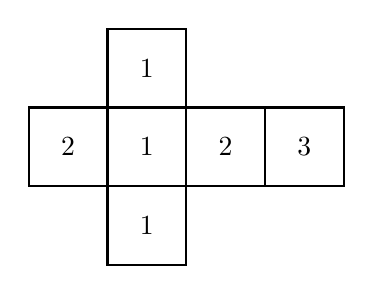
\begin{tikzpicture}[
]
	\draw (0,0) node{2};
	\draw (1,0) node{1};
	\draw (1,1) node{1};
	\draw (1,-1) node{1};
	\draw (2,0) node{2};
	\draw (3,0) node{3};
	\draw[thick] (-0.5,-0.5) -- (3.5,-0.5) -- (3.5,0.5) -- (-0.5,0.5)--cycle;
	\draw[thick] (0.5,-1.5) -- (1.5,-1.5) -- (1.5,1.5) -- (0.5,1.5)--cycle;
	\draw[thick] (2.5,-0.5)--(2.5,0.5);
\end{tikzpicture}
}
\begin{abienum}[start=3]

	\item In einem Zufallsversuch wird der nebenstehende Würfel zweimal geworfen. 

	\begin{abienum}
		\item Stellen Sie den o.g. Sachverhalt in einem Wahrscheinlichkeitsbaum mit allen Pfadwahrscheinlichkeiten dar. \phantom{x}~\hfill\textbf{(5BE)}
		\item Erläutern Sie an diesem Sachverhalt die Begriffe Ergebnis und Ereignis eines Zufallsversuchs. ~\hfill\textbf{(3BE)}
		\item Nennen Sie die Definitionen der Begriffe Zufallsgröße und binomialverteilte Zufallsgröße und geben Sie jeweils eine binomialverteilte bzw. eine nicht-binomialverteilte Zufallsgröße für diesen Zufallsversuch an. ~\hfill\textbf{(5BE)}
	\end{abienum}
	\end{abienum}
\end{rightgraphic}



\begin{abienum}[start=4]
\item In einem weiteren Zufallsversuch wird der Würfel insgesamt 100-mal geworfen. Bestimmen Sie die Wahrscheinlichkeiten dafür, dass die Augenzahl 3

	 \begin{enumerate}[label=\Alph*:]
 	\item genau 10-mal
 	\item höchstens 10-mal
 	\item mindestens 20-mal 
   \end{enumerate} 

   geworfen wird. ~\hfill\textbf{(4BE)}

\item Es soll überprüft werden, ob der o.g. Würfel gezinkt wurde. Ein Mitschüler schlägt vor, den Würfel 50 mal zu werfen. Wird die Augenzahl 3 mindestens 10 mal gewürfelt, entscheidet man, dass der Würfel gezinkt ist. Nehmen Sie Stellung zu diesem Vorschlag. ~\hfill\textbf{(9BE)}


\end{abienum}


\newpage

{\large \textbf{\textsf{Material}}}

\textbf{\textsf{Material 1:}}

\begin{tikzpicture}[
]
\begin{axis}[schule,
	xlabel=t,
	%ylabel=y,
	x=0.2cm,
	y=0.0002cm,
	%xtick distance=1,
	%ytick distance=1,
	xmin=0,
	xmax=42,
	ymin=0,
	ymax=37000,
	scale ticks above exponent={5}
]
	\addplot [domain=0:45, black] {36000/(1+35*e^(-0.25*x))};
	\addplot [domain=0:45, red] {1000*1.10^x};
	\addplot [domain=0:45, blue] {36000-35000* e^(-0.105*x)};


	\node[below left] (0) at (0,-2pt) {\scriptsize $0$};
\end{axis}
\end{tikzpicture}

\newpage

\begin{landscape}

 \textbf{\textsf{Erwartungshorizont/Protokoll}}
 \scriptsize

\SetTblrTemplate{head}{empty}
\SetTblrTemplate{foot}{empty}
 \begin{longtblr}{	
  width    = \linewidth,
  colspec  = {l|X[l]|X[l]|X[l]},
  rowhead  = 1,
  hline{even} = {0.5pt,solid},
  hline{odd} = {0pt,solid},
  row{even}    = {4cm},
  row{odd} = {lightgray},
  cells = {valign = h},
  hlines,
 	vlines
}

% Header row (repeated)
\textbf{Nr} & \textbf{Erwartungshorizont}      & \textbf{Schülerleistung Vortrag}      & \textbf{Schülerleistung Kolloquium}      \\ 

1.1 & {f-rot: exponentielles (unbeschränktes) Wachstum \\
g-blau: beschränktes Wachstum\\
h-schwarz: logistisches Wachstum
} &  &  \\
& \textbf{BE: 3/3/0} & & \\ 
1.2 & {
	f: Es handelt sich um (unbeschränktes) exponentielles Wachstum. Der Anfangsbestand beträgt 1000 und der Wachstumsfaktor 1,1 (Wachstum um 10\% auf 110\%)\\[0.5cm]
	g: Es handelt sich um beschränktes Wachstum.\\
	Der Anfangsbestand beträgt 36000-35000=1000.\\
	$e^{-0,105t}≈0,9^t$. Die Anzahl der Nichtinfizierten beträgt zu Beginn 35000 und reduziert sich wöchentlich um 10\% auf 90\% (exp. Zerfall der Nichtinfizierten). Langfristig nähert sich der Bestand der Sättigungsgrenze von 36000.\\[0.5cm]
	h: Es handelt sich um logistisches Wachstum. Dies hat auch die Sättigungsgrenze 36000. Das Wachstum beginnt beim Anfangsbestand von 1000. Dieser steckt im Term $35=\frac{36000}{1000}-1$. Das logistische Wachstum beginnt zunächst mit langsamer Geschwindigkeit, steigert sich bis zum Wendepunkt und flacht dann mit Näherung an die Sättigungsgrenze immer weiter ab. 
}  &  &  \\
& BE: \textbf{0/6/0} & & \\ 
1.3 & {
	Es handelt sich bei der in der Aufgabenstellung beschriebenem Wachstum um ein beschränktes Wachstum $g(t)$. 
	Die 10\% der Nichtinfizierten, die jede Woche neu infiziert werden, entsprechen einer Abnahme der Nichtinfizierten auf 90\%.
}  &  &  \\
& BE: \textbf{2/0/0} & & \\ 
2.1 & {$18000= 36000 - 35000 \cdot e^{-0,105t}$\\[0.2cm]
	$18000=35000\cdot e^{-0,105t}$\\[0.2cm]
	$\dfrac{18}{35}=e^{-0,105t}$\\[0.2cm]
	$\ln(\dfrac{18}{35})=-0,105t$\\[0.2cm]
	$t=-\dfrac{\ln(\dfrac{18}{35})}{0,105}≈6,3331$\\[0.2cm]
	Nach 6 Wochen und 3 Tagen (Nach 6,3 Wochen) ist die Hälfte der Bevölkerung erkrankt.
}  &  &  \\
& BE: \textbf{1/3/0} & & \\ 
2.2 & {$g'(t)=3675\cdot e^{-0,105t}$\\[0.5cm]
	$g'(t)$ beschreibt einen exponentiellen Zerfall. Die Funktion ist monoton fallend. Daher ist am linken Rand des Definitionsbereichs der Funktionswert maximal.
}  &  &  \\
& BE: \textbf{2/2/0} & & \\ 
2.3 & { $G(t)=36000t+\frac{1000000}{3}e^{-0,105t}$\\[0.5cm]
$0,1\cdot\pint{g(t)}{0}{10}{t}=0,1\cdot(G(10)-G(0))≈0,1\cdot(476645,9-333333,3)=14331,26$\\[0.5cm]
In den ersten zehn Wochen beträgt die durchschnittliche Zahl der Infizierten ca. 14331.	
}  &  &  \\
& BE: \textbf{0/5/0} & & \\ 
2.4 & { $36000 - 35000 \cdot e^{-0,105t}=36000$ \\
$- 35000 \cdot e^{-0,105t}=0$\\
$e^{-0,105t}=0$\\
Die Exponentialfunktion nimmt nie den Funktionswert 0 an. Daher hat die Gleichung keine Lösung. Die Funktion nähert sich der 0 aber beliebig nah an. Daher ist im Anwendungskontext irgendwann auch der letzte Nichtinfizierte infiziert worden.
}  &  &  \\
& BE: \textbf{0/2/3} & & \\ 
2.5 & {z.B. Ansatz $g(t)=36000 - 35000 \cdot e^{-0,105t}=35999,1$\\
$t\approx 100,6$\\
Nach ca. 100 Wochen.
}  &  &  \\
& BE: \textbf{0/0/2} & & \\ 	
3.1 & {
	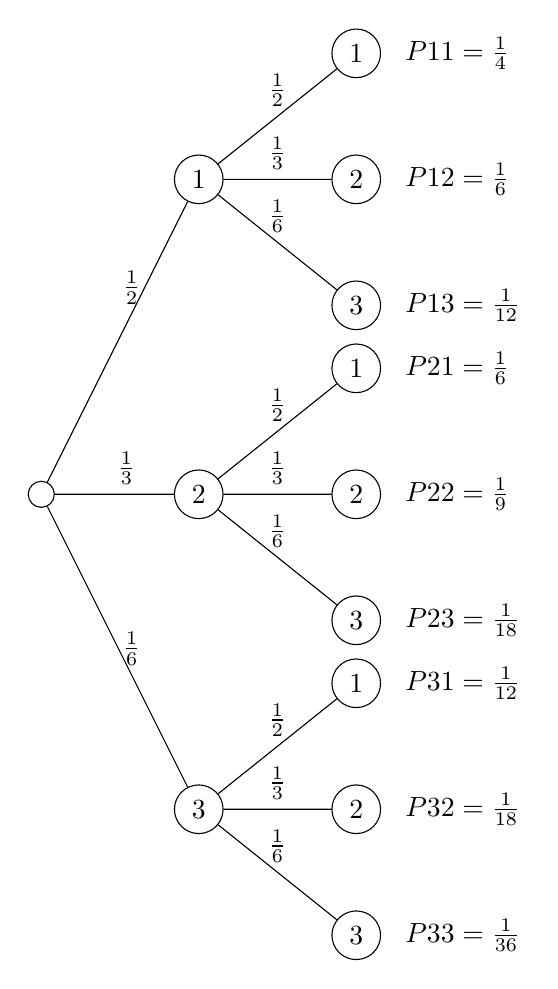
\begin{tikzpicture}[grow=right]

\tikzstyle{level 1}=[level distance=2cm, sibling distance=4cm]
\tikzstyle{level 2}=[level distance=2cm, sibling distance=1.6cm]
\node[circle,draw] (0) {$$}
	child {node[circle,draw] (R) {3}
			child {node[circle,draw] (RR) {3} edge from parent node[above, pos=0.5] {$\frac{1}{6}$}}
			child {node[circle,draw] (RG) {2} edge from parent node[above, pos=0.5] {$\frac{1}{3}$}}
			child {node[circle,draw] (RB) {1} edge from parent node[above, pos=0.5] {$\frac{1}{2}$}}
		edge from parent node[above, pos=0.6] {$\frac{1}{6}$}}
	child {node[circle,draw] (G) {2}
			child {node[circle,draw] (GR) {3} edge from parent node[above, pos=0.5] {$\frac{1}{6}$}}
			child {node[circle,draw] (GG) {2} edge from parent node[above, pos=0.5] {$\frac{1}{3}$}}
			child {node[circle,draw] (GB) {1} edge from parent node[above, pos=0.5] {$\frac{1}{2}$}}
		edge from parent node[above, pos=0.6] {$\frac{1}{3}$}}
	child {node[circle,draw] (B) {1}
			child {node[circle,draw] (BR) {3} edge from parent node[above, pos=0.5] {$\frac{1}{6}$}}
			child {node[circle,draw] (BG) {2} edge from parent node[above, pos=0.5] {$\frac{1}{3}$}}
			child {node[circle,draw] (BB) {1} edge from parent node[above, pos=0.5] {$\frac{1}{2}$}}
		edge from parent node[above, pos=0.6] {$\frac{1}{2}$}};
	
	\node[right] at ([xshift=0.5cm] BB) {$P\pr{11} = \frac{1}{4}$};
	\node[right] at ([xshift=0.5cm] BG) {$P\pr{12} = \frac{1}{6}$};
	\node[right] at ([xshift=0.5cm] BR) {$P\pr{13} = \frac{1}{12}$};
	\node[right] at ([xshift=0.5cm] GB) {$P\pr{21} = \frac{1}{6}$};
	\node[right] at ([xshift=0.5cm] GG) {$P\pr{22} = \frac{1}{9}$};
	\node[right] at ([xshift=0.5cm] GR) {$P\pr{23} = \frac{1}{18}$};
	\node[right] at ([xshift=0.5cm] RB) {$P\pr{31} = \frac{1}{12}$};
	\node[right] at ([xshift=0.5cm] RG) {$P\pr{32} = \frac{1}{18}$};
	\node[right] at ([xshift=0.5cm] RR) {$P\pr{33} = \frac{1}{36}$};
\end{tikzpicture}
}  &  &  \\
& BE: \textbf{5/0/0} & & \\ 	
 3.2 &{
 	Die Ergebnisse sind in diesem Experiment die Tupel $S=\{(1,1),(1,2),(1,3),(2,1),(2,2),(2,3),(3,1),(3,2),(3,3)\}$. Ein Ereignis ist eine Teilmenge der Ergebnismenge und besteht aus keinem, einem oder mehreren Ergebnissen. Ein mögliches Ereignis ist „Pasch“ $E=\{(1,1),(2,2),(3,3)\}$.
 }  &  &  \\
 & BE: \textbf{0/3/0} & & \\ 
 3.3 & {Eine Zufallsgröße ist eine Funktion, die jedem Ergebnis eine reelle Zahl zuordnet. Beispiel für eine nicht binomialverteilte Zufallsgröße ist die Augensumme. Bei einer binomialverteilten Zufallsgröße müssen die folgenden Eigenschaften gelten:\\[0.5cm]
 \begin{minipage}{\hsize}
 \begin{itemize}
 	\item Ein Experiment wird wiederholt. Die Wahrscheinlichkeiten ändern sich nicht.
 	\item Ein Teil der Ergebnisse zählt als „Erfolg“.
 	\item Die Zufallsgröße zählt die Anzahl der Erfolge.
 \end{itemize}
 \end{minipage}\\[0.5cm]
 Beispiel: Anzahl der 3er.
 } &  &  \\
 & BE: \textbf{0/5/0} & & \\ 
 4.&{$P(A)=B(100;1/6;10)≈0,0214$\\[0.5cm]
 	$P(B)=F(100;1/6;10)≈0,0427$\\[0.5cm]
 	$P(C)=1-F(100;1/6;19)≈0,2197$
 }  &  &  \\
  & BE: \textbf{0/4/0} & & \\ 
 5.& {Grundsätzlich prüft der Test auf der rechten Seite, ob die Wahrscheinlichkeit für 3 größer ist als 1/6. Eine Verminderung der Wahrscheinlichkeit wäre aber ebenfalls denkbar. Daher müsste ein zweiseitiger Test durchgeführt werden.\\
 	$P(X\geq 10)=1-F(50;1/6;9)≈0,3170$\\
 	Der Fehler 1. Art, also den Würfel fälschlicherweise als gezinkt einzustufen, wäre mit 32\% relativ groß.\\
 	Zweiseitiger Hypothesentest mit $\alpha=0,05$\\
 	$F(50;1/6;3)=0,0238$\\
 	$F(50;1/6;4)=0,0643$\\
 	$F(50;1/6;13)=0,9692$\\
 	$F(50;1/6;14)=0,9861$\\
 	$P(X\leq k_1)\leq 0,025 \Rightarrow k_1=3$\\
 	$P(X\geq k_2) \leq 0,025 \Rightarrow k_2=14$\\
 	Annahmebereich $A={4,5,\ldots,13}$
 } &  &  \\
   & BE: \textbf{0/0/9} & & \\ 
 &  &  &  \\
 &  &  &  \\
 &  &  &  \\
 &  &  &  
\end{longtblr}
	
\end{landscape}

\begin{tblr}{
  colspec={|l|X[c]|X[c]|X[c]|c|},
  width=\linewidth,
  row{1-2} = {font=\bfseries},
  row{Z} = {font=\bfseries},
  column{5} = {font=\bfseries},
  cell{1}{2} = {c=3}{c},
  hlines,
  vlines
}
Aufgabe & \shortstack{Bewertungseinheiten in den\\ Anforderungsbereichen} & & & Summe \\
        & AFB I & AFB II & AFB III &        \\
1.1     & 3     & 3       &         & 6      \\
1.2     &      &  6     &         & 6      \\
1.3     &    2  &       &         & 2      \\
2.1     &    1   & 3      &        & 4      \\
2.2     &   2    & 2      &         & 4      \\
2.3     &       & 5      &         & 5      \\
2.4     &       &   2     &  3     & 5      \\
2.5     &      &       &  2       & 2      \\
3.1     &  5    &       &        & 5      \\
3.2     &      & 3      &         & 3      \\
3.3     &       &  5      &        & 5      \\
4   & &4 &  & 4\\
5   & & & 9 & 9\\
Summe   & 13    & 33     & 14      & 60     \\
\end{tblr}


Prüfungsergebnis von 5 Punkten (ausreichend) setzt voraus, dass insgesamt 45\% der zu vergebenen BE erreicht werden. Der Prüfling stellt seine/ihre Ergebnisse überwiegend in einem verständlichen Vortrag in einfacher Sprache dar. Weiterführende Fragen im Prüfungsgespräch werden in vergleichbaren Umfang in den AFB I-II beantwortet. 

Ein Prüfungsergebnis von 11 Punkten (gut) setzt voraus, dass insgesamt 75\% der zu vergebenden BE erreicht werden. Der Prüfling stellt seine/ihre Ergebnisse in einem fließenden freien und strukturierten Vortrag mit sicherer und korrekter Verwendung der Fachbegriffe dar. Weiterführende Fragen im Prüfungsgespräch werden in vergleichbaren Umfang in den AFB II-III beantwortet.

\newpage

{\large \textbf{\textsf{Zusatzfrage A}}}

Für das Modell $h(t)== \dfrac{36000}{1+35e^{-0,25t}}$ gilt für die Ableitungsfunktion $h'(t)$ der folgende Zusammenhang:

$h'(t)=r\cdot h(t) \cdot \left(36000 - h(t)\right)$, wobei $r$ eine positive Konstante ist.

\begin{itemize}
	\item Bestimmen Sie den Wendepunkt von $h(t)$.
	\item Geben Sie den Wert von r an.
	\item Zeigen Sie, dass für die zweite Ableitung $h''(t)$ gilt:

	$h''(t)=r\cdot h'(t)\cdot \left( 36000 - 2\cdot h(t) \right)$
\end{itemize}

{\large \textbf{\textsf{Zusatzfrage B}}}

Die Abbildung zeigt den Graphen einer in $\mathbb{R}$ definierten,
differenzierbaren Funktion $g(x)$.

Betrachtet wird eine in $\mathbb{R}$ definierte Funktion $f(x)$, für deren erste Ableitungsfunktion 

$f'(x)=e^{g(x)}$ gilt.

\begin{itemize}
	\item Untersuchen Sie, ob der Graph von f einen Extrempunkt hat.
	\item Untersuchen Sie, ob der Graph von f einen Wendepunkt hat.
\end{itemize}

\begin{tikzpicture}[
]
\begin{axis}[schule,
	xlabel=x,
	ylabel=y,
	%x=0.2cm,
	%y=0.0002cm,
	%xtick distance=1,
	%ytick distance=1,
	%xmin=0,
	%xmax=42,
	%ymin=0,
	%ymax=37000,
	%scale ticks above exponent={5}
]
	\addplot [domain=-5:8, black] {(x+4)*e^(-0.4*x)};

	\node[below left] (0) at (0,-2pt) {\scriptsize $0$};
\end{axis}
\end{tikzpicture}

{\large \textbf{\textsf{Zusatzfrage C}}}

Skizzieren Sie den Graphen von $f(x)=\cos (\frac{1}{2}\cdot x)+1$ im Intervall $[0;4\pi ]$. 

Begründen Sie ohne Verwendung einer Stammfunktion, dass

$\pint{\left(\cos\left(\frac{1}{2}\cdot x\right)+1\right)}{0}{2\pi}{x}=2\pi\cdot 2\cdot \dfrac{1}{2}=2\pi$ gilt.



\end{document}